\chapter{Results and discussion}

% \section{Introduction}

% Abbreviations what should be included? FDA?

% Small planar molecules have the ability to intercalate between consecutive DNA basepairs altering the structure of DNA locally and at a larger scale. This effect can lead to mutations and the erroneous functioning of the DNA in living organism. Exploiting this effect has lead to a number of drugs and drug candidates due to their anti-cancer effects. FDA approved drugs like <blank> etc. have proven effect in treating some forms of cancer. ~Despite their widespread use, the mechanism of binding has not been completely established.~ \emph{Put something about how there are not enough}. 
% 
% It has been shown previously that binding affinity are correlated with the efficacy of a drug molecule (along with other factors like ADME). Binding affinity for protein ligand systems are now calculated routinely both in academia and industry with validation and predictive power. Alchemical free energy methods coupled with accelerated sampling predict the binding affinity of a wide range of protein-ligand systems with accuracies of less then \SI{1}{\kilo\calorie\per\mol} in a consistent manner.



% Put it in context.

% Furthermore DNA-intercalator systems have been probed by computational methods relatively less compared to protein-ligand systems.

% Don't use quinoaline 

% Propuse of thsi paper: three methods used to calualtion


% \section{Methods}

% Models

% We are looking at intercalators that are bound between two consecutive base pairs and not minor or major groove binders.

% Two data-sets: one for validating docking, the other for the free energy calculations methods. 

% Docking

% Give details about parameters, how you define the docking box, etc.
% What is the direction of the intercalators, conformations, scoring.

% Future work (end of conclusion or discussion or mention it in results when comparing to experiment talking about possibilities why these are the best results. Temperature, concentration, pH, conformation, length of base pair.)
% Intercalation between other sequences.

% \section{Results}

% The title subsections have to have title about what you used the methods for, not what the method is that you used!


% Use passive pls. 

This chapter describes and discusses the results. The results for each of the computational approaches to estimate either the binding free energy directly or range the intercalators is presented first, followed by a discussion of their relative merits.


\section{Docking and scoring}

% Introduce the intercalators
% Talk about the crystal structures that you found. How, where etc.

% TODO: check what is the nomenclature for a DNA-intercalator system/crystal structure

% Purpose of this section. Why there are nine intercalators here and why are we doing this?

The rigid planar scaffold of the intercalators that bind between DNA basepairs reduces the possible number of conformations that the docked structure can have. We have shown that using an extensive search method for docking, intercalators can be docked with RMSD less than $1$ angstrom for a wide range of intercalators compared to crystal structures.

We collected nine crystal structures of DNA-intercalator complex where the intercalator is between two consecutive basepairs. Table~\ref{tab:docking} shows the RMSD of every intercalator docked compared to the crystal structure. For seven of the cases docking is very close to the crystal structure, with average RMSD of $0.76$ angstrom. There are two cases where the docked structure is far from the reference.

After further investigating the outlier, the docked intercalators are in the correct place between the two basepairs, but their orientation is different from the one in the reference crystal structure. If there is no symmetry present in the intercalator molecule, then there are four possible orientations once docked. The free energy difference between these orientations is probably low, and the experimentally observed, dominant orientation is dependent of the kinetics of the intercalation too.

The quinoxaline scaffold based intercalators were also docked and scored into the basepair opening of the 1Z3F crystal structure removing the original intercalated molecules. 

% 
\begin{table}[h]
  \caption{Results of docking nine intercalators compared to crystal structures.}
  \label{tab:docking}
  \centering
  \begin{tabular}{lS[round-mode=figures,round-precision=2]}
  \toprule
  {PDB ID} & {RMSD [angstrom]} \\
  \midrule
  1Z3F &  5.527405 \\
  1Z3F &  0.833399 \\
  1G3X &  0.593967 \\
  1HX4 &  1.195613 \\
  2ROU &  3.920575 \\
  1D11 &  0.586476 \\
  1D11 &  0.871855 \\
  1D12 &  0.401521 \\
  1D12 &  0.856238 \\
  \bottomrule
  \end{tabular}
\end{table}


\section{ESMACS}

In the past, there has been a number of MMPBSA type calculations for DNA intercalator systems. A large majority of these studies only takes into account just a few (one to three) intercalators binding to the DNA, and does not compare to experimental studies. We obtained a correlation Pearson coefficient of $r_p=0.70$ across the 10 planar molecules for the 3 trajectory calculation.

\subsubsection{Convergence}

It is important to assess the sampling efficiency and converge of the predicted free energy values in order for the results to be reliable and reproducible.
First, the comparison in convergence between a single trajectory approach and an ensemble of trajectories is compared for the MMPBSA and NMODE analysis methods in the context of free energy calculations. As the improvement in ensemble methods was evident, we investigated the length of each replica, extending the simulations from the original 5 ns simulation to 20 ns for each of the 25 replicas. It was important to sample the system long enough to cover a large part of the phase space, but not to oversample in places where the methods is no longer valid, for example during a de-intercalation pathway.

\subsubsection{Replica size and bootstrapped error}



\begin{figure}
  \begin{tikzpicture}
\begin{axis}[
  xlabel=Number of replicas,
  ylabel={Error (kcal/mol)},
  ]
  
  \addplot table {bootstrap.csv};
  
\end{axis}
\end{tikzpicture}
  \caption{Bootstrapped error as a function of replica size. }
  \label{fig:bootstrap}
\end{figure}

\subsubsection{Predicting the ranking}

The experimental free energy values are between \SIlist{-3.69;-3.50}{\kilo\calorie\per\mole}, making them hard to differentiate computationally. Approximate methods, like ESMACS, that are based on MMPBSA and NMODE for the free energy and entropy contribution, respectively do not have the resolution to differentiate experimental values at this scale. Nonetheless, correct error control and ensemble based calculations can give meaningful results relative to each other, i.e. ranking the intercalators based on their free energies will be comparable to experimental ranking.

% In methods talk about 1, 2, 3 trajectory

We have run 1, 2 and 3 trajectory calculations and as seen in Figure~\ref{fig:mmpbsa} the correlation improves, with the 3 trajectory being the most accurate with a correlation coefficient of $r_p=0.70$. The small interval of the experimental values suggests that the intercalators are very closely binding to the DNA. 

% This is a new subsection describing the energy components. P
% Check the 

The correlation achieved with ESMACS in this study suggests that one of the underlying forces (electrostatic, vdW, or internal energy) dominates the interaction gradient between the intercalators, and that signal is picked up by the MMPBSA calculation. Figure~\ref{fig:corrmat} shows the spread of the free energy values of the different components. Previous studies \cite{} have shown that vdW interactions contribute most to the binding energy of the intercalators in absolute terms. However, the correlation of the different components to the total binding energy shows that the internal energy (the sum of bond, angle, and torsion terms) correlate ~surprisingly~ with the total. 
% Induce fit, what it is?
This further supports our claim that the intercalation is an induced fit inside the two base-pairs.

% Methods
Each ESMACS calculation was run 25 times, the only difference being the random seed at the start of the simulation. 

% Beginning, quality of simulations, 
Variations in the results from the different replica was used to evaluate the error on the predicted free energy. Figure~\ref{fig:bootstrap} shows the bootstrapped error as a function of the number of replicas. There is a leveling off at around 20 replicas, with 25 replicas showing consistently low error bars.

% Energy contribution section
NMODE analysis was performed to include an approximation to the entropy contribution. Results show that including NMODE does not improve the ranking. 

% Convergence

% The original ESMACS protocol by \cite{} et al. 

\begin{figure}[h!]
	\documentclass[margin=0.1in]{article}

\usepackage{pgfplots}
\usepackage{pgfplotstable}
\pgfplotsset{compat=newest}


\usepackage{amsmath}
\usepackage{tikz}
\usetikzlibrary{positioning, calc}

\pgfmathsetmacro{\s}{0.5}
\pgfmathsetmacro{\r}{0.5cm}

\usepackage[caption=false]{subfig}

\begin{document}

\begin{figure}
  
\subfloat{%
\begin{tikzpicture}%3traj
\begin{axis}[
  scale=0.7,
  xtick distance = {0.1},
  ytick distance = {1},
  %xlabel={\phantom{nothing}}, 
  %ylabel={Calculated $\Delta$G (\si{\kilo\calorie\per\mole})},
  legend pos=south east]
  
  \addplot[blue!70!white] table [col sep=comma, x=exp, y={create col/linear regression={y=dg_3_traj}}] {4-ring-mmpbsa.csv};
  % \addplot[red!70!white] table [col sep=comma, x=exp, y={create col/linear regression={y=dg_3_traj_nmode}}] {4-ring-mmpbsa.csv};

  \addplot[blue, mark=*, only marks, error bars/.cd,
          x dir=both, x explicit,
          y dir=both, y explicit,] table 
          [col sep=comma, x=exp, y=dg_3_traj, y error=dg_3_traj_err, x error=exp_err] {4-ring-mmpbsa.csv};
  % \addplot[red, mark=*, only marks, error bars/.cd,
  %         x dir=both, x explicit,
  %         y dir=both, y explicit,] table[col sep=comma, x=exp, y=dg_3_traj_nmode, y error=dg_3_traj_err, x error=exp_err] {4-ring-mmpbsa.csv};
  
  \legend{3 trajectory, $R=0.70$}%, w/ n-mode}

\end{axis}  
\end{tikzpicture}%
}
\subfloat{%
\begin{tikzpicture}%3traj-nmode
\begin{axis}[
  scale=0.7,
  xtick distance = {0.1},
  ytick distance = {1},
  %xlabel={\phantom{nothing}}, 
  %ylabel={Calculated $\Delta$G (\si{\kilo\calorie\per\mole})},
  legend pos=south east]
  
  \addplot[red!70!white] table [col sep=comma, x=exp, y={create col/linear regression={y=dg_3_traj_nmode}}] {4-ring-mmpbsa-failednmode.csv};
  % \addplot[red!70!white] table [col sep=comma, x=exp, y={create col/linear regression={y=dg_3_traj_nmode}}] {4-ring-mmpbsa.csv};

  \addplot[red, mark=*, only marks, error bars/.cd,
          x dir=both, x explicit,
          y dir=both, y explicit,] table 
          [col sep=comma, x=exp, y=dg_3_traj_nmode, y error=dg_3_traj_err, x error=exp_err] {4-ring-mmpbsa-failednmode.csv};
  % \addplot[red, mark=*, only marks, error bars/.cd,
  %         x dir=both, x explicit,
  %         y dir=both, y explicit,] table[col sep=comma, x=exp, y=dg_3_traj_nmode, y error=dg_3_traj_err, x error=exp_err] {4-ring-mmpbsa.csv};
  
  \legend{3 trajectory + nmode, $R=0.62$}%, w/ n-mode}

\end{axis}  
\end{tikzpicture}
}

\subfloat{%
\begin{tikzpicture}%2traj
\begin{axis}[
  scale=0.7,
  xtick distance = {0.1},
  ytick distance = {1},
  %xlabel=Experimental $\Delta$G (\si{\kilo\calorie\per\mole}), 
  %ylabel={Calculated $\Delta$G (\si{\kilo\calorie\per\mole})},
  legend pos=south east
  ]
  
  \addplot[blue!70!white] table [col sep=comma, x=exp, y={create col/linear regression={y=dg_2_traj}}] {4-ring-mmpbsa.csv};    
  % \addplot[red!70!white] table [col sep=comma, x=exp, y={create col/linear regression={y=dg_2_traj_nmode}}] {4-ring-mmpbsa.csv};

  \addplot[blue, mark=*, only marks, only marks, error bars/.cd,
          x dir=both, x explicit,
          y dir=both, y explicit,] table[col sep=comma, x=exp, y=dg_2_traj, y error=dg_2_traj_err, x error=exp_err] {4-ring-mmpbsa.csv};
  % \addplot[red, mark=*, only marks, only marks, error bars/.cd,
  %         x dir=both, x explicit,
  %         y dir=both, y explicit,] table[col sep=comma, x=exp, y=dg_2_traj_nmode, y error=dg_2_traj_err, x error=exp_err] {4-ring-mmpbsa.csv};
  \legend{2 trajectory, $R=0.64$}%, w/ n-mode}

\end{axis}  
\end{tikzpicture}%
}
\subfloat{%
\begin{tikzpicture}%2traj-nmode
\begin{axis}[
  scale=0.7,
  xtick distance = {0.1},
  ytick distance = {1},
  %xlabel=Experimental $\Delta$G (\si{\kilo\calorie\per\mole}), 
  %ylabel={Calculated $\Delta$G (\si{\kilo\calorie\per\mole})},
  legend pos=south east
  ]
  
  \addplot[red!70!white] table [col sep=comma, x=exp, y={create col/linear regression={y=dg_2_traj_nmode}}] {4-ring-mmpbsa-failednmode.csv};    
  % \addplot[red!70!white] table [col sep=comma, x=exp, y={create col/linear regression={y=dg_2_traj_nmode}}] {4-ring-mmpbsa.csv};

  \addplot[red, mark=*, only marks, only marks, error bars/.cd,
          x dir=both, x explicit,
          y dir=both, y explicit,] table[col sep=comma, x=exp, y=dg_2_traj_nmode, y error=dg_2_traj_err, x error=exp_err] {4-ring-mmpbsa-failednmode.csv};
  % \addplot[red, mark=*, only marks, only marks, error bars/.cd,
  %         x dir=both, x explicit,
  %         y dir=both, y explicit,] table[col sep=comma, x=exp, y=dg_2_traj_nmode, y error=dg_2_traj_err, x error=exp_err] {4-ring-mmpbsa.csv};
  \legend{2 trajectory + nmode, $R=0.50$}%, w/ n-mode}

\end{axis}  
\end{tikzpicture}
}

\subfloat{%
\begin{tikzpicture}%1traj
\begin{axis}[
  scale=0.7,
  xtick distance = {0.1},
  ytick distance = {1},
  %xlabel={\phantom{nothing}}, 
  %ylabel={Calculated $\Delta$G (\si{\kilo\calorie\per\mole})},
  legend pos=south east
  ]
  
  \addplot[blue!70!white] table [col sep=comma, x=exp, y={create col/linear regression={y=dg_1_traj}}] {4-ring-mmpbsa.csv};    
  % \addplot[red!70!white] table [col sep=comma, x=exp, y={create col/linear regression={y=dg_2_traj_nmode}}] {4-ring-mmpbsa.csv};

  \addplot[blue, mark=*, only marks, only marks, error bars/.cd,
          x dir=both, x explicit,
          y dir=both, y explicit,] table[col sep=comma, x=exp, y=dg_1_traj, y error=dg_1_traj_err, x error=exp_err] {4-ring-mmpbsa.csv};
  % \addplot[red, mark=*, only marks, only marks, error bars/.cd,
  %         x dir=both, x explicit,
  %         y dir=both, y explicit,] table[col sep=comma, x=exp, y=dg_2_traj_nmode, y error=dg_2_traj_err, x error=exp_err] {4-ring-mmpbsa.csv};
  \legend{1 trajectory, $R=0.64$}%, w/ n-mode}
\end{axis}  
\end{tikzpicture}%
}
\subfloat{%
\begin{tikzpicture}%1traj-nmode
\begin{axis}[
  scale=0.7,
  xtick distance = {0.1},
  ytick distance = {1},
  %xlabel={\phantom{nothing}}, 
  %ylabel={Calculated $\Delta$G (\si{\kilo\calorie\per\mole})},
  legend pos=south east
  ]
  
  \addplot[red!70!white] table [col sep=comma, x=exp, y={create col/linear regression={y=dg_1_traj_nmode}}] {4-ring-mmpbsa-failednmode.csv};    
  % \addplot[red!70!white] table [col sep=comma, x=exp, y={create col/linear regression={y=dg_2_traj_nmode}}] {4-ring-mmpbsa.csv};

  \addplot[red, mark=*, only marks, only marks, error bars/.cd,
          x dir=both, x explicit,
          y dir=both, y explicit,] table[col sep=comma, x=exp, y=dg_1_traj_nmode, y error=dg_1_traj_err, x error=exp_err] {4-ring-mmpbsa-failednmode.csv};
  % \addplot[red, mark=*, only marks, only marks, error bars/.cd,
  %         x dir=both, x explicit,
  %         y dir=both, y explicit,] table[col sep=comma, x=exp, y=dg_2_traj_nmode, y error=dg_2_traj_err, x error=exp_err] {4-ring-mmpbsa.csv};
  \legend{1 trajectory + nmode, $R=0.39$}%, w/ n-mode}
\end{axis}  
\end{tikzpicture}
}
\end{figure}

\end{document}
	\caption{Correlation between one (bottom), two (middle) and three (top) trajectory calculations and experiment. Values are presented for NMODE (red) analysis and without NMODE (blue). The best Pearson correlation is for the NMODE-less values starting from \num{0.64} for the 1, and 2 trajectory and \num{0.70} for the 3 trajectory. The NMODE calculations have a Pearson correlation of \numlist{0.39; 0.5; 0.62} for the 1, 2, and 3 trajectory calculations respectively.}
	\label{fig:mmpbsa}
\end{figure}


\section{TIES}

Relative alchemical free energy calculations were done between five pairs of the intercalator from the original experimental study. As discussed above, there are two groups of intercalator there: the four and five membered ring scaffolds. Pairs were selected based on two criteria: first to maximise the experimental free energy difference and second to sample all three possible combinations of transformation (between the 4 ring systems, 5 ring systems, and a transformation from 4 ring to 5 ring). 

As seen in figure~\ref{fig:ties} the correlation to experiment is poor. This can be for a number of reasons, but investigating more systems could be insightful. The experimental results for this study indicate binding affinities that are very close to each other, and even the best methods will struggle to differentiate between them. In the future we will collect and simulate intercalator ligand systems with experimental free energy differences large enough to be probed computationally. The simulations do converge as seen in figure~\ref{fig:ties_conv} well before the end of the simulation time. Still, TIES does produce more accurate results then the more approximate methods like ESMACS or docking. The root mean squared error on this small set of transformations is 0.41 kcal/mol.

\begin{figure}
  \centering
  \begin{tikzpicture}
\begin{axis}[
  ylabel=Predicted $\Delta \Delta G$,
  xlabel=Experimental $\Delta \Delta G$,
  ]
  
  \addplot[blue, mark=*, only marks] table {ties.csv};
  
\end{axis}  
\end{tikzpicture}
  \caption{Correlation plot comparing the experiment free energy difference with the calculated values via TIES. The experimental values are too close to each other, and the difference is smaller than the resolution of the TIES method given the 5 replicas used here. Furthermore the experimental error becomes large when we take the free energy difference between two values.}
  \label{fig:ties}
\end{figure}

\begin{figure}
  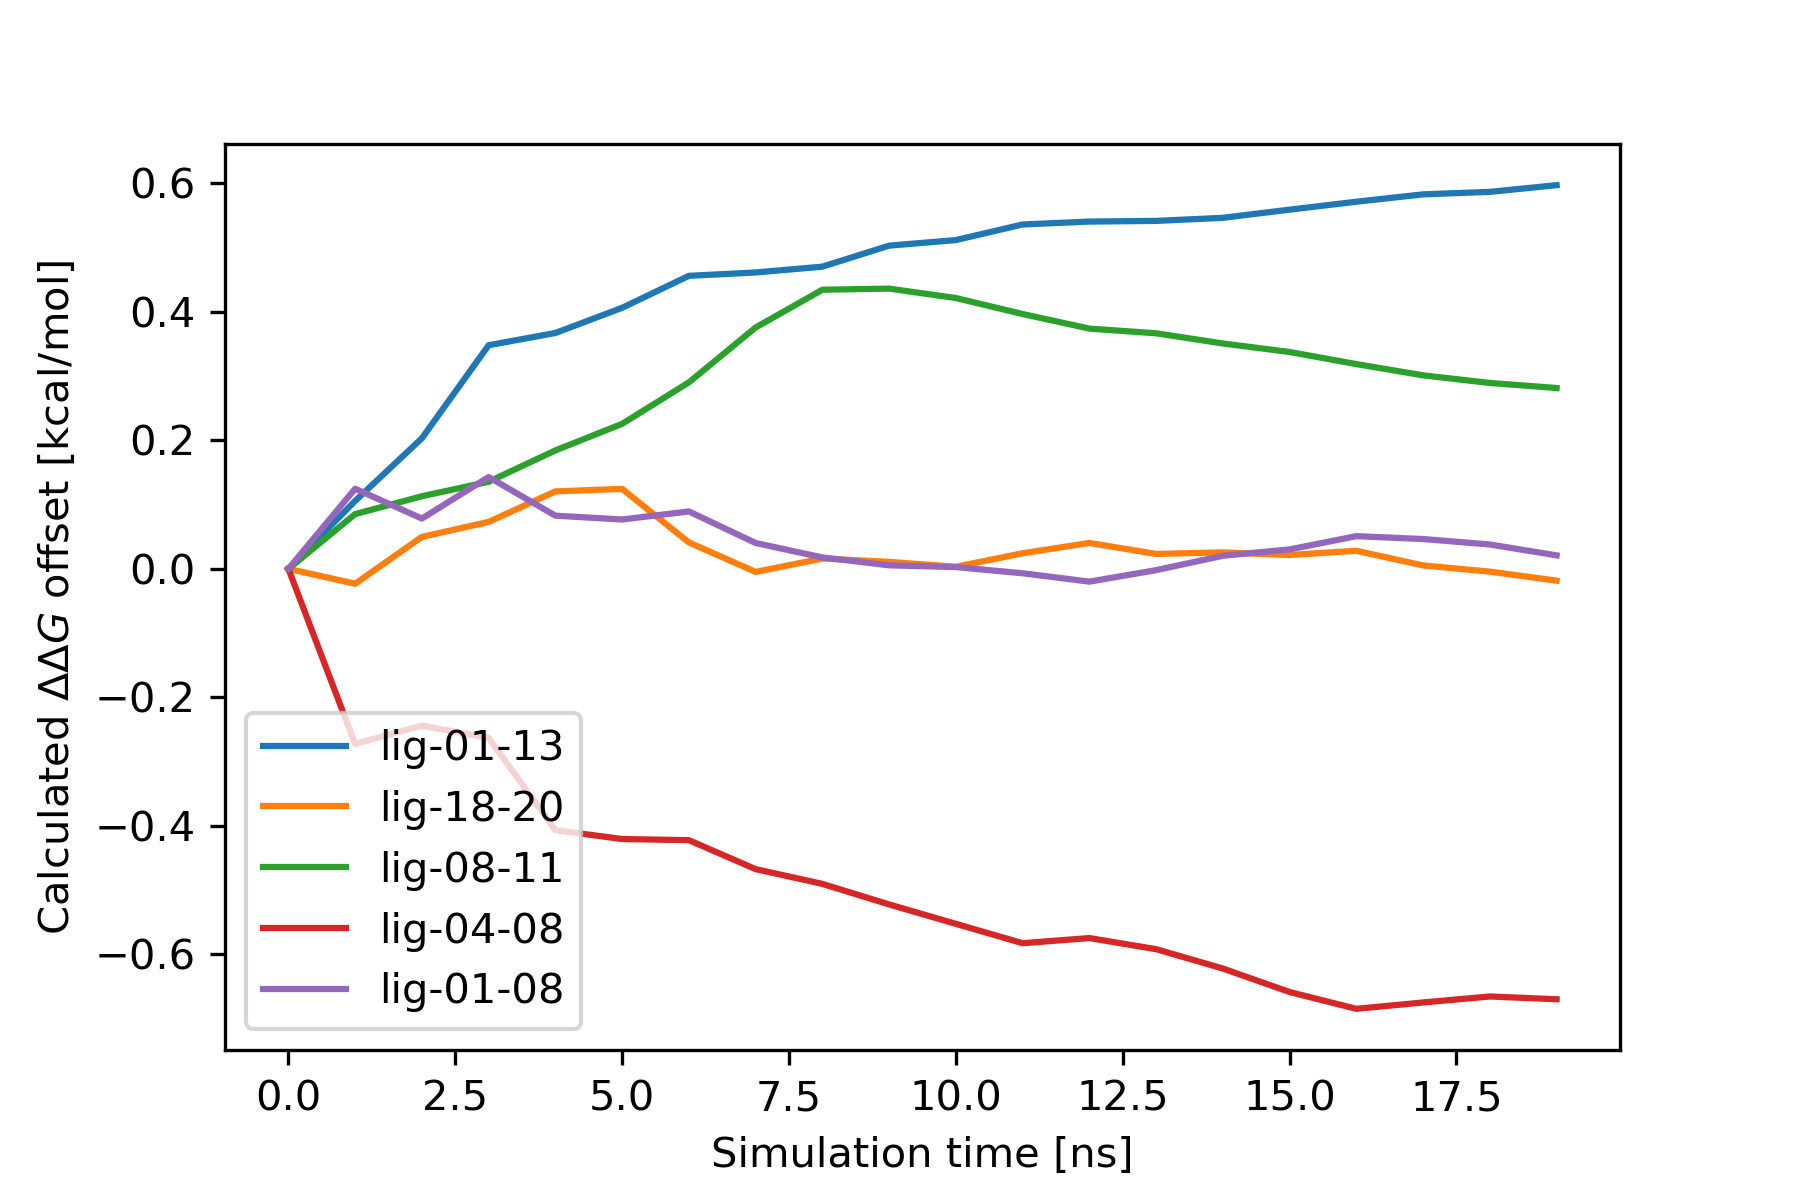
\includegraphics[width=\columnwidth]{ties_conv.png}
  \caption{Time evolution of the free energy difference for the five intercalator pairs investigated. The results are levelled off indicating that we reached converged values. The values are offset so they all start at point zero for illustrative purposes.}
  \label{fig:ties_conv}
\end{figure}



\section{Discussion}

The three methods we investigated correspond to three theoretically more accurate ways of quantifying the relative or absolute binding affinity of these intercalators. 

